% ==============================================================================
% Section 4.5: Sex Disaggregation (RQ4)
% ==============================================================================
\subsection{Sex Disaggregation (RQ4)}
\label{sec:sex}

As documented in Section~\ref{sec:data}, the four outcome statuses differ substantially in their sex composition.
We now examine whether these aggregate differences translate into distinct spatial clustering patterns.

Figure~\ref{fig:sex_maps} compares male and female LISA maps for Not Located and Located Dead in \referencemonth{}.

\begin{figure}[htbp]
  \centering
  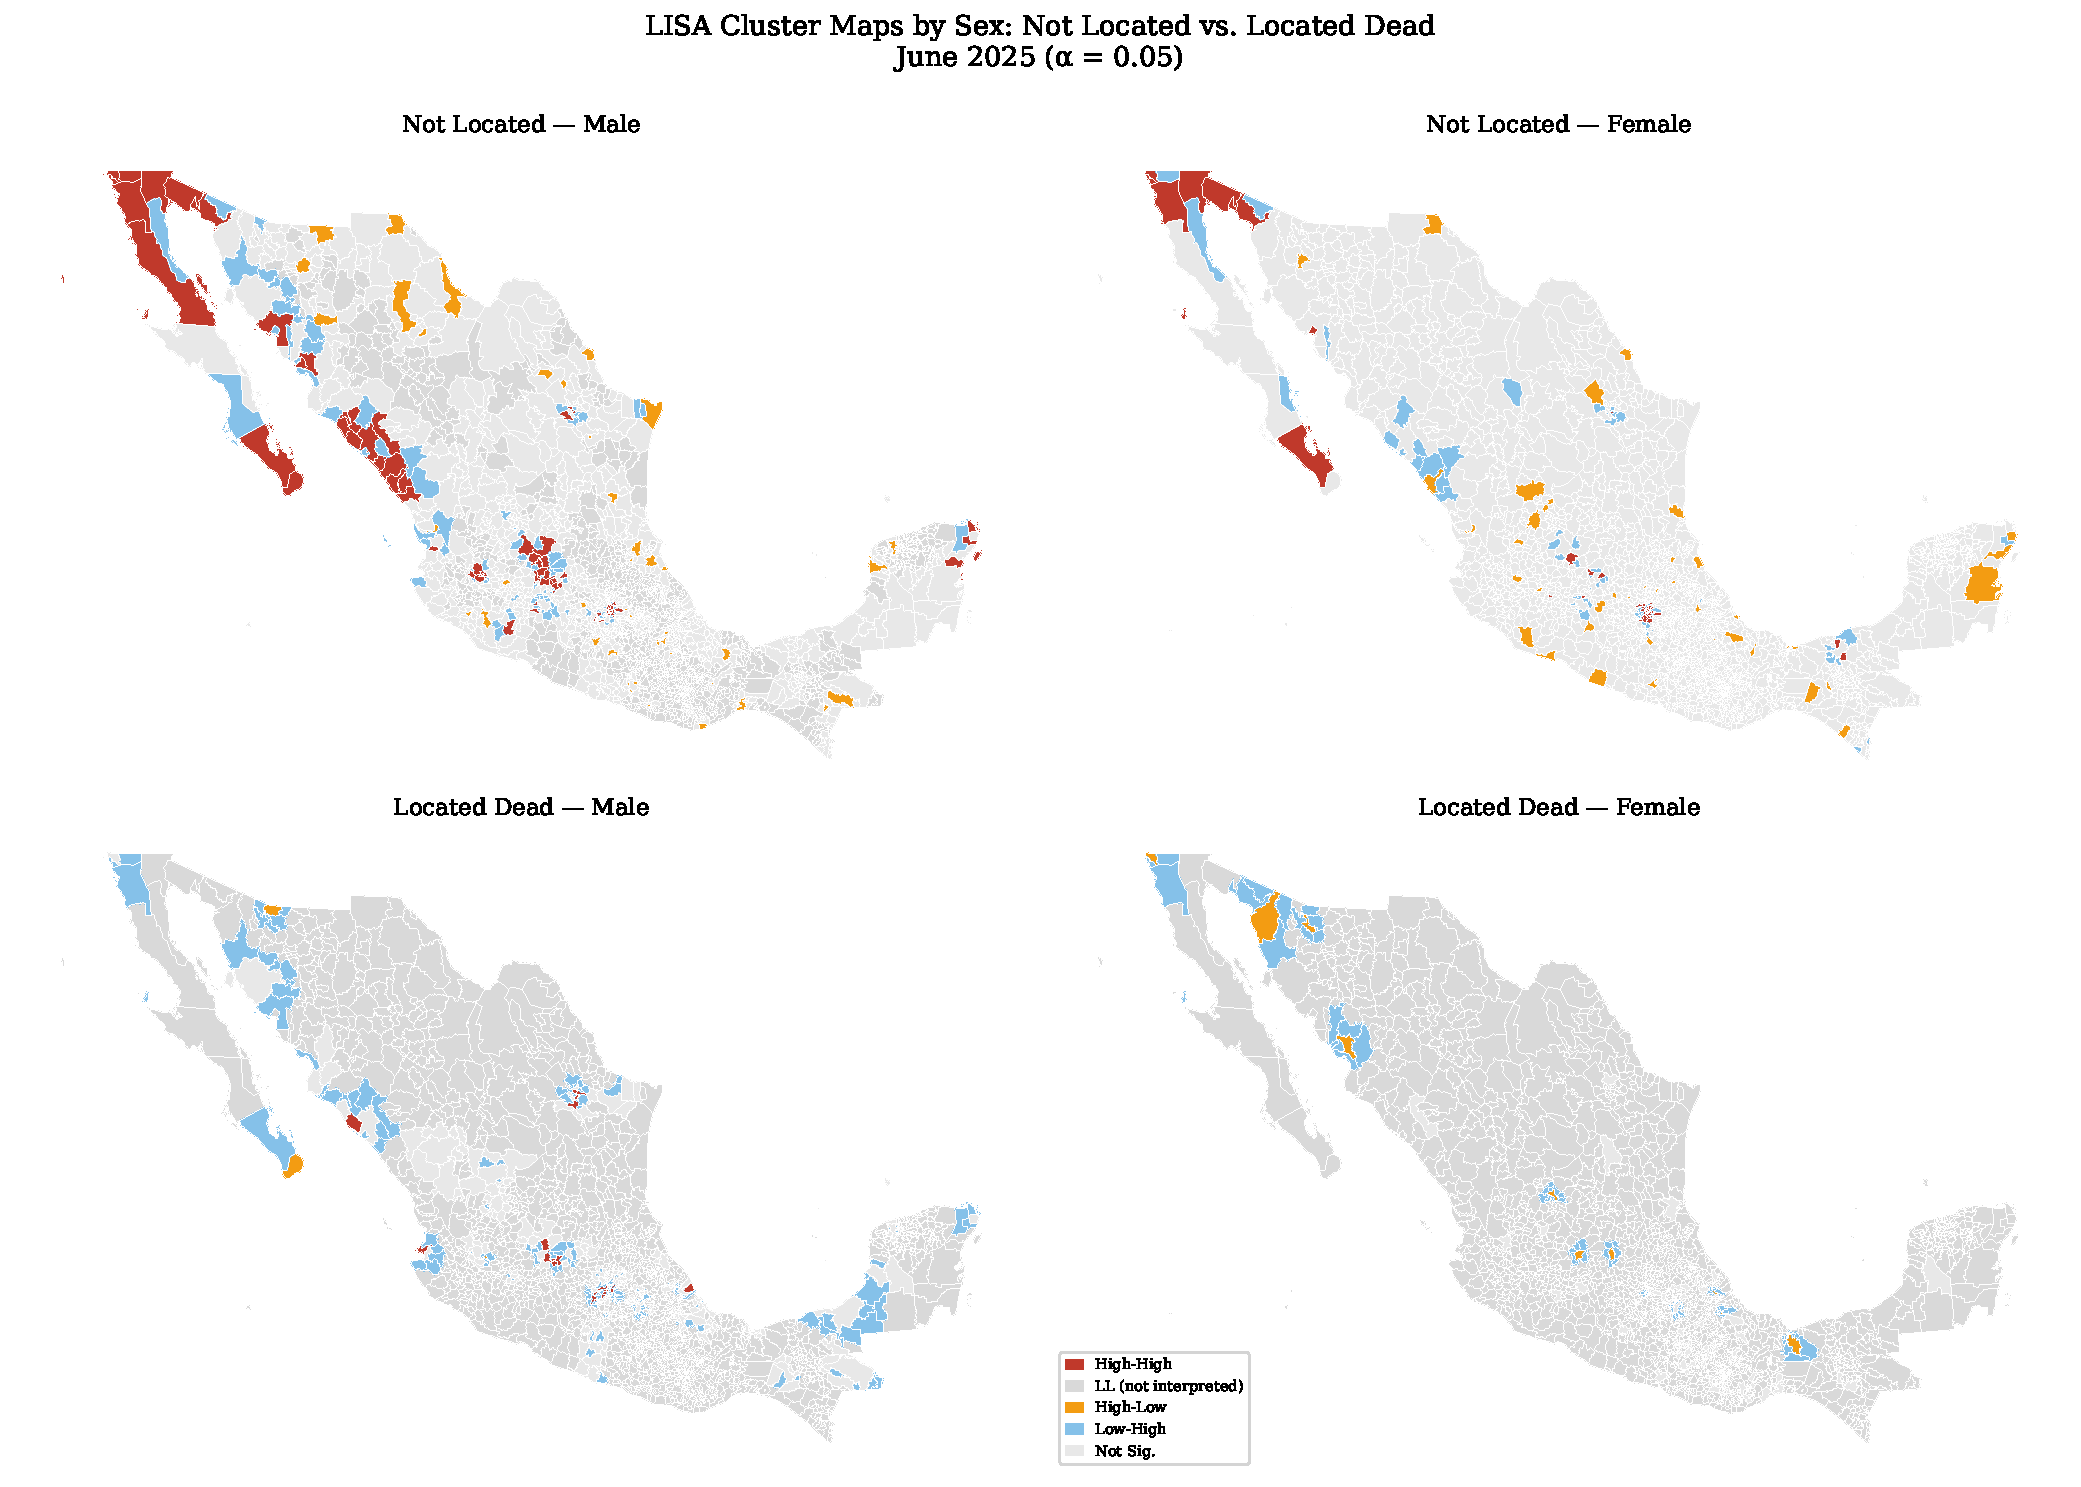
\includegraphics[width=\textwidth]{figures/fig7_sex_disaggregation_maps.pdf}
  \caption{LISA cluster maps by sex for Not Located (top) and Located Dead (bottom),
           \referencemonth{}.
           Left = male; right = female. Projection: EPSG:6372.}
  \label{fig:sex_maps}
\end{figure}

Table~\ref{tab:sex} quantifies the overlap between male and female HH classifications.

\begin{tabular}{lrrrrrr}
  \toprule
  \textbf{Status} & \textbf{Total HH} & \textbf{Male HH} & \textbf{Female HH} & \textbf{M $\cap$ F} & \textbf{M only} & \textbf{F only} \\
  \midrule
  Total & 80 & 84 & 73 & 55 & 29 & 18 \\
  Not Located & 71 & 66 & 40 & 23 & 43 & 17 \\
  Located Alive & 93 & 68 & 82 & 49 & 19 & 33 \\
  Located Dead & 17 & 15 & 0 & 0 & 15 & 0 \\
  \bottomrule
  \multicolumn{7}{l}{\footnotesize Reference period: June 2025. $\alpha=0.05$, Queen contiguity, 999 permutations.} \\
  \multicolumn{7}{l}{\footnotesize M $\cap$ F = municipalities HH under both male and female LISA. M/F only = sex-exclusive hotspots.} \\
\end{tabular}

For Total, 121 municipalities are classified as male HH and 99 as female HH, with 74 municipalities classified as HH for both sexes (Jaccard = 0.507).
Located Alive shows a similar pattern: 83 male HH, 90 female HH, and 58 shared (Jaccard = 0.504).
The moderate Jaccard values indicate that roughly half of the hotspot geography is shared, while the remainder is sex-specific.

Not Located exhibits greater divergence: 85 male HH versus 50 female HH, with only 28 shared municipalities (Jaccard = 0.262).
The lower female count reflects the male-dominated sex composition of Not Located cases (77.9\% male); fewer municipalities generate sufficient female-only counts to reach HH significance.
The low overlap suggests that the few municipalities with concentrated female Not Located cases are not the same municipalities driving male Not Located clustering.

Located Dead presents the starkest result: 27 male HH municipalities but \emph{zero} female HH municipalities (Jaccard = 0.000).
This is not a substantive finding about gendered victimization geography; it is a statistical power failure.
With a mean of 0.0065 female Located Dead cases per municipality-month and 99.4\% of cells recording zero, the LISA algorithm lacks sufficient spatial variation to detect any clusters.
Female Located Dead results should be excluded from policy interpretation.
